%!TEX root = ../paper.tex

\section{Survey}
\label{sec:survey}

As described in Section~\ref{sec:introduction}, the authors of this paper share a strong belief that source code history is commonly used for program understanding tasks and that there is a lack of tool support for these tasks. In order to examine to what degree this belief can be confirmed in practice, we created an extensive online survey for professional developers. In particular, we were seeking answers to the following research questions:

\begin{enumerate}[label=\textbf{RQ\arabic*}, labelindent=\parindent, listparindent=\parindent]
	\item Do developers use source code history when they are working with code? If so, what are they trying to learn when they examine source code history?
	\item In terms of their mental models and information needs, what level of temporal and structural granularity are most appropriate when using source code history?
	\item How do developers identify the history of specific code units and how well does existing tooling support them?
	\item Does augmenting history with semantic data improve program comprehension? How effectively can a semantical-aware code history viewer support program comprehension?\fg{I asked myself repeatedly now what the difference between 'semantic' and 'semantical' could be. I guess it's time for a clarification...}
\end{enumerate}

\noindent Answers to these questions from a set of professional developers would provide us a much better picture in regard to the feasibility of our idea of a semantic source code history tool.

\subsection{Survey Design}
\label{sec:survey-design}

Our online survey consisted of four parts and a total of 18 questions among which some were based on example scenarios described in the survey. Questions were either free text or likert-scale as shown in the example in Figure\ref{fig:example_likert_question}. Additionally, we asked participants for background information in regard to their current job position, development experience and the version control tools they use. The survey started after participants gave consent on the first page and could be paused and resumed any time. We estimated an average of 20 minutes for completion. The survey was structured as follows\footnote{The full survey can be seen here: XXX}:

\begin{figure}[t!]
  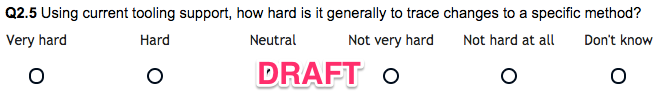
\includegraphics[width=0.98\columnwidth]{figures/example_likert_question}
  \caption{Example likert-scale question}
  \label{fig:example_likert_question}
\end{figure}

\textbf{Part 1} was designed to convey a general picture in regard of RQ1-2. We tried to provide a gentle entry and asked for the recency and a description of the participant's last activity with source code history (RQ1). To investigate the structural granularity (first part of RQ2) we let participants rate how interested they are in history at different levels, e.g. \textit{file}, \textit{class/module}, \textit{field/variable}, \textit{method/function}, \textit{block}. In terms of the temporal granularity (second part of RQ2) we asked for a description on how far in the past they normally examine history and how they decide for this time span.

\textbf{Part 2} first provided a brief scenario in line with the one described in Section~\ref{sec:scenario_general}: a developer is faced with a pull request and wants to understand better what the code that was changed is actually doing. Using this scenario, we wanted to gain more information about whether developers use source code history for program understanding tasks and what information they are searching for (RQ1). We first asked participants how familiar this scenario appears to them and then for a description of how they would approach this problem. We then isolated the imaginary change to a change to a \textit{single method} and asked participants how they would identify changes in history that changed this method as an example of a semantic unit. We asked subsequently how well the participant's described strategy would cope with complex structural changes to this method (e.g. renaming, moving to a different file). Concluding Part 2, we asked how hard it is generally to trace changes to a method with current tooling support and for a description of what makes this hard or easy. Responses would provide us a clear picture on whether developers struggle with the tools they use for purposes as in the scenario (RQ3).

\textbf{Part 3} then moved on to a practical instance of the general scenario from Part 2 on Github\footnote{XXX}. We created a sample pull request\footnote{XXX} in our forked repository of the \textit{Checkstyle} project described in Section~\ref{sec:motivation} that changed a specific method. We provided a link to the associated file history\footnote{XXX} and asked participants to describe how they would identify commits in this history that changed the method of interest. While we expected that the challenge of this task would become visible from these descriptions we also asked directly how well existing tools support this task (RQ3). With this background, we moved towards RQ4 and let participants rate how useful a semantic history (i.e. history of this method only) would be in this scenario and how hard it would be to find the commit that really introduced the sample method (e.g. in the face of multiple refactoring operations).

Where Parts 1-3 of the survey investigated in the potentials of a semantic history tool with both general questions and a specific scenario, \textbf{Part 4} showed for the first time what the output of such a tool \textit{could} look like. We mocked an output for the scenario in Part 3, showing the respective commits and diffs that changed the method alongside detailed descriptions of the changes in natural language. To inform RQ4 and the feasibility of our approach further, we now asked for a rating on (a) how helpful this output would be for a better understanding of the method, (b) how hard it would be to retrieve this type of information manually and (c) how valuable a tool would be that could generate this output. Finally, we gave participants the option to express what other information could have been valuable that was not in our mocked result view.

\fg{I have a feeling that readers who haven't seen our survey will not yet get a good enough picture of it with this description. Maybe we could think about illustrating the sample scenarios and especially our mocked output somehow. But I'm not sure.} 

\subsection{Participants}
\label{sec:survey-participants}

% Q5.1-Q5.6: (questions on participants' backgrounds)

We recruited XXX professional developers from industry (XXX) and academia (XXX). Participants were selected and contacted individually from the authors' professional networks. For this survey, we traded a large pool of participants (e.g. with advertisement of anonymous links) in favor of certainty of participants' professional backgrounds in order to avoid misleading responses due to lack of experience. The majority of job titles (XXX\%) were \textit{software developer/engineer} or analogical terms. The remaining XXX\% were academic positions like \textit{PHD student}, \textit{researcher} or \textit{professor}. XXX\% had more than 4 years of programming experience (XXX\% > 10 years) and XXX\% had been professional software developers for more than 4 years (XXX\% > 10 years). XXX\% had used source code history for more than 4 years (XXX\% > 10 years). Figure~\ref{fig:popular_tools} shows our participants' most frequently used source code history tools. Other tools mentioned were specific IDE's and their add-ons with JetBrains IDEs (IntelliJ/PHPStorm/WebStorm) being most present, followed by VSCode and Eclipse. A few other tools (e.g. GitLens, GitKraken) were mentioned as well, but were not very common. In our view, the XXX responses convey an expressive and generalizale impression on developers' relationships with source code history.

\begin{figure}[t!]
  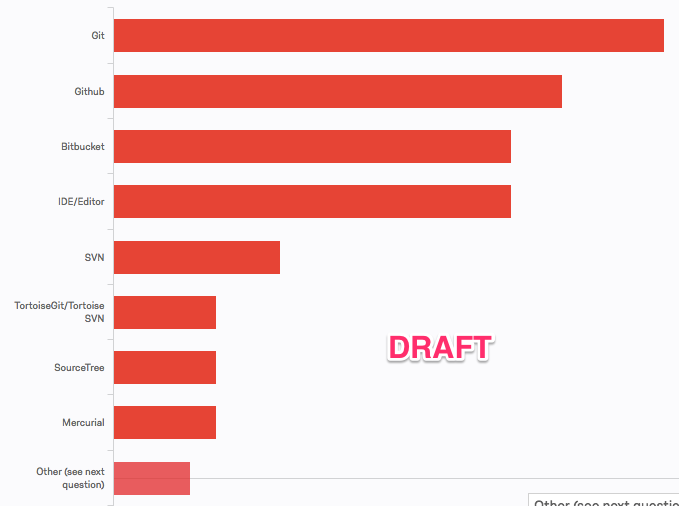
\includegraphics[width=0.98\columnwidth]{figures/popular_tools}
  \caption{Most popular source code history tools}
  \label{fig:popular_tools}
\end{figure}

\subsection{Survey Results}
\label{sec:survey-results}

We summarize and categorize the results of our survey in sequence of the research questions.

% ===================================================
% =================== RQ1 ===========================
% ===================================================

\mybox{\textbf{RQ1: }Do developers use source code history when they are working with code? If so, what are they trying to learn when they examine source code history?}

% Q1.1: How recently did you last use source code history of any kind?
% Q1.2: Please describe this most recent activity. How did you use source code history? What were you looking for? Did you find it? Did the tools you used support you in this investigation or could they be improved?

\noindent
The great majority of our participants use source code history very frequently: prior to the survey, XXX\% of participants had used source code history within two days prior to performing the survey (XXX\% < 1 week, XXX\% < one month). When asked for a description of this most recent activity, we first observe many common version control tasks, e.g. ``push some changes'', ``tagging the repo for a release'', ``merge branches'' or ``check what I modified''. We can also see many activities associated with accountability; participants checked ``who had been contributing'', ``who [they] could contact for dev support'' and ``who is associated with some changes''.

However, we can also deduce a big fraction of activities related to program understanding. Participants wanted to ``understand how the solution to a certain problem was implemented'' and ``how and why [a property] was changed''. Some participants were generally interested in the ``evolving of software architecture'' and in ``what steps a certain component took to get to the shape/position it was in''. The term \textit{understand} appeared XXX times when participants described their most recent activity.

Moreover, it becomes visible that developers search and navigate extensively through source code history to ``find reasons for [...] changes''. Participants ``browsed for a change made by a specific commit in the history'', ``[looked] for a specific change that might have introduced an issue'' and ``[looked] for an outdated implementation of a functionality''. They tried to ``[figure] out [a] history of changes'' and ``[compared] files over multiple commits''. The terms \textit{looked}, \textit{browsed}, \textit{searched} and \textit{navigated} appeared XXX times in the descriptions of most recent activities.

% Q2.1: Does this scenario sound familiar to you (i.e. have you encountered this in the past)?
% Q2.2: Please describe very briefly how you would approach this problem. What kinds of questions would you like to answer? What tools or approaches would you use to answer them?

When asked how familiar participants were with our scenario of a developer being faced with a pull request, not knowing what the code is actually doing, XXX\% replied with \textit{very familiar} or \textit{familiar}. When asked for a description of their strategy in this scenario, most participants replied that in a majority of cases their first step would be to approach the pull request author because ``they have to be accountable''. Other frequent strategies were to refer to issue trackers because they would tell ``what were the design decisions that lead to the change''. Other documentation from both within the pull request and external was also mentioned repeatedly, especially if the author is unavailable. Many developers would ``run that version locally and step through the different functions using a debugger'' because the pull request ``must contain a detailed setup to build an exact test environment''. Testing was another important topic and participants would be ``running the tests'' and inspect whether the change would ``cause any tests to change their fail/pass status''.

We can see that version history tools are another source of information and in fact the first step for some: ``my first step would be to look at the code history'' or ``fire up the history view [...] and hope for the best''. However, in comparison to other strategies (asking the author, documentation, tests, running changes locally), source code history would be used less frequently in this scenario\fg{because it's not good enough?!}.

% ===================================================
% =================== RQ2 ===========================
% ===================================================

\mybox{\textbf{RQ2: }In terms of their mental models and information needs, what level of structural and temporal granularity are most appropriate when using source code history?}

% Q1.3: In terms of source code granularity, how interested are you in gathering information on source code history at the following levels?

\noindent
Figure~\ref{fig:structural_granularity} shows how interested our participants were in gathering information on source code history at different levels of \textit{structural granularity}. We can see that developers are generally at least somewhat interested in all levels with the categories 'Neutral', 'Not very interested' and 'Not interested at all' having very low percentages. The most significant levels of interest were \textit{Method/Function} and \textit{Class/Module} with both having around XXX\% in the categories 'Very interested' and 'Interested'. This shows that developers are in fact mainly interested in the history of semantic code units rather than traditional, file- and text-based structural levels like \textit{File} or \textit{Directory/Package}, having only XXX\% and XXX\% in these categories respectively.

\begin{figure}[t!]
  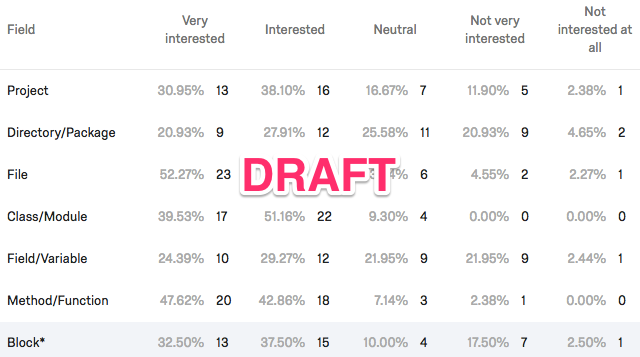
\includegraphics[width=0.98\columnwidth]{figures/structural_granularity}
  \caption{Structural granularity most appropriate when using source code history}
  \label{fig:structural_granularity}
\end{figure}

% Q1.4: When you use code history, how far in the past do you usually examine? How do you determine how far in the past you want to go?

To examine the \textit{temporal granularity} we asked participants how far in the past they usually examine and how they determine how far they want to go. The responses were mostly consistent in a way that ``this largely depends on the goal'' and that the time range can be very diverse because the fragment of interest is based on changes and commits rather than time. But there is also a clear thread that participants ``don't usually go [back] more than a few weeks'' or ``a couple of days'' in most cases, but at other times they ``look at the commit history years ago''. Interestingly, the cases where they examine further in the past seem to be related to program understanding tasks most often, e.g. when ``looking for the reason for a code change'', ``if some functionality seems odd or obsolete while reviewing source code'' or ``to understand why and how specific parts became the way they are today''.

% ===================================================
% =================== RQ3 ===========================
% ===================================================

\mybox{\textbf{RQ3: }How do developers identify the history of specific code units? How effectively does existing tooling support them?}

% Q2.3: Using source code history, how would you find changes to this method only? Please describe briefly.
% Q2.5: Using current tooling support, how hard is it generally to trace changes to a specific method?

\noindent
With the example code unit of a \textit{method} we referred back to our general pull request example and asked our participants how they would \textit{generally} identify the history of a method and how challenging this task is. We identified \textit{file history} as the most important strategy. Some participants described how they would limit the history to isolate changes to a method, e.g. using a combination of \texttt{git log} and \texttt{grep}. Many also mentioned recursive or iterative calls to \texttt{git blame} and more high-level sources of information like commit messages and issue trackers. To our surprise, only very few mentioned line- and range-based history, i.e. \texttt{git log -L} and higher-level abstractions like \textit{Show history for selection/method} in IntelliJ. Many participants immediately described this task as ``not trivial'', ``not easy'' and ``not the funniest job''  when asked for their strategy. Rating the difficulty of the task in a later question, XXX\% chose \textit{hard} or \textit{very hard}, XXX\% chose \textit{neutral}, and XXX\% chose \textit{not very hard} or \textit{not hard at all}.

% Q2.4: How well would your strategy cope with more complex structural changes, e.g. method renaming, moving of a method, refactoring?
% Q2.6: Given your answer to the previous question (Q2.5), what makes this hard or easy?

Figure~\ref{fig:strategy_complex_changes} shows participants' ratings of how well their strategies cope with more complex structural changes. It is visible that the change types \textit{method renames} and \textit{signature changes} are coped with quite well, but also that \textit{split into multiple methods} and especially \textit{move to different file} (XXX\% \textit{not very well} or \textit{not well at all}) are very hard to cope with. This is strongly confirmed by the responses to our question what would make this hard or easy where the main notion was that it depends on the complexity of changes: ``It's either easy (the method hasn't undergone complex changes) or challenging (the method has undergone complex changes). When it is challenging, it is VERY difficult.'' Many participants mentioned specifically that ``not knowing the semantics'' and the fact that ``[there] is no direct or explicit abstraction to method/class levels'' makes it very hard.

\begin{figure}[t!]
  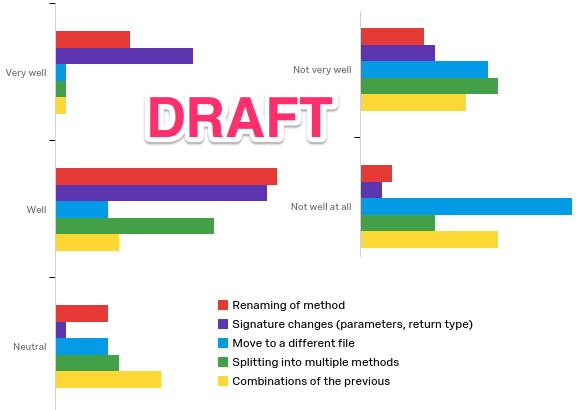
\includegraphics[width=0.98\columnwidth]{figures/strategy_complex_changes}
  \caption{How well do participants' strategies cope with more complex structural changes?}
  \label{fig:strategy_complex_changes}
\end{figure}

% Q3.1: In the above version history, how would you identify the commits in which the method of interest has changed? Please describe your strategy briefly.

When faced with our real-world example from the \textit{Checkstyle} repository \fg{I was just wondering here if it would be a lot better maybe if we could refer back to the example in the motivation. But it's not the example from the survey anymore. The example is better, but we're losing the connection to the survey a bit. Something to discuss.} and the associated file history, our participants assessed the task of identifying commits that changed the method as even more challenging than in the general previous questions. While some were quite plain that they can't think of a strategy for this scenario (``I have no idea how I would do this'', ``Not at all'', ``I sincerely have no idea''), we can see others who would come up with more advanced strategies like ``write a script'' or a ``divide and conquer mechanism'' but that this ``seems overkill''. But generally, we can see most participants falling back to the history of the file containing the method and they ``would dig through the history to find the method in each commit'' and ``open each one of them and manually inspect''. Some immediately pointed out the limits of this strategy: ``[if] the method comes from another class [...], that would be more difficult to trace'' and that ``it's annoying'', ``you got me with this one'', ``there's too much garbage noise'' and the ``revisions are too many to go through''. Some expressed unawareness of whether ``there is any tool that allows [them] to track the function across commits''.

% Q3.2: How well do existing tools support identifying these changes?
% Q3.4: How hard would it be to find the first commit for the given method and whether the method was really created then or if it was moved there from somewhere else (e.g. through a file renaming, or through a refactoring)?

When asked how well existing tools support identifying these changes, no participant said \textit{very well}, XXX\% said \textit{well} and XXX\% said \textit{neutral}. The great majority of participants rated with either \textit{not very well} or \textit{not well at all} (XXX\%). When asked how hard it would be to find the first commit that really introduced the method (rather than being just a refactoring commit), XXX\% replied with \textit{hard} or \textit{very hard}. 

% ===================================================
% =================== RQ4 ===========================
% ===================================================

\mybox{\textbf{RQ4: }Does augmenting history with semantic data improve program comprehension? How effectively can a semantic-aware code history viewer support program comprehension?}

% Q3.3: How useful would it be to have support for a more semantic history in this scenario (e.g. history for this method or class only)?
% Q4.1: Consider again the described situation of being faced with a pull request for a change of a method. How helpful would you consider the information above for getting a better understanding of the method and its history?
% Q4.2: How hard would you consider retrieving information on the history of a method with the above level of detail?
% Q4.3: If a tool could generate information in the fashion of the above on any method or other code unit, how valuable would you consider this tool?

\noindent
We mentioned previously that some participants mentioned that specifically the lack of semantic awareness of history tools makes it hard to trace the changes of methods (``not knowing the semantics''). When we now asked specifically how useful it would be to have support for a more semantic history for our example scenario  (i.e. history for this method only), XXX\% replied with \textit{very useful} or \textit{useful}. Participants were now faced with our mocked output of a fictitious semantic history tool, showing change descriptions and the commits and diffs that changed the method. When asked how valuable they would consider a tool generating this output automatically, XXX\% replied with \textit{very valuable} or \textit{valuable} and XXX\% consider retrieving this information manually \textit{hard} or \textit{very hard}. When asked how helpful they would consider this information for a better understanding of the method being faced with the pull request, XXX\% replied with \textit{very helpful} or \textit{helpful}. 

% Q4.4: What other information that is not in the descriptions above would you consider valuable?
% Q5.7: Do you have any final comments? Do you have any other ideas for tool support or systems to solve the general problems described in this survey and its scenarios? Is there anything else on your mind?

The generally positive attitute towards our idea was expressed explicitly by some when we asked for other information that could be valuable and in the final comments: ``having the information above would be a big improvement in the daily business'' and it would be great ``to generate a method-, class-, file-history/protocol in a human-readable way'' and to have ``version control that was method-aware, or aware of classes/modules''. As indicated before in RQ2, our \textit{method} example code unit was confirmed as ``definitely the best use case'' by some. However, some developers were ``not sure [they] would find rich method-level semantics that useful'' and to very few the usage of history for the described scenarios was overall unintuitive: ``why/how would I need/use history; to blame people for bugs?''. A few confirmed that ``the history of a [code unit] helps to understand a pull request, but [they] usually don't find the need to do so''. Some also expressed that ``it is not something I miss in my daily work but of course it would be very helpful in these rare situations where tracking [of code units] is needed''. Other responses also indicate that this more critical feedback - of history being not very useful for program understanding - may be ``because the tools that [they] use don't support this feature''. Some even thanked us that the survey helped them realized ``that [they] use VCS purely as an archive''.

We can deduce three main groups of other information that participants would find valuable that we did not present in our mocked semantic history outputs. First and foremost was \textit{authorship and intent}: developers seem to be highly interested in the question ``who made the changes and why''. While some commented that ``this is available in the linked commits so not really missing'', others regarded our output as just ``information when and what changed''. Along the same lines, many participants mentioned information from issue trackers associated with the changes being missing. Second was \textit{references}: many participants responded that ``it would be interesting to see where [a method]'s (been) used (in the past)'' and specifically ``the call reference to this method which in turn has been refracted just because of this method change''. Third was \textit{associated tests}: participants were interested in ``associated test runs/suites'' influenced by the change to the code unit because ``this would help to know if the methods were changed to fix specific bugs, or if they were refactored in an attempt to cleanup code''. We will discuss these suggestions more in Section~\ref{sec:discussion}.


